\chapter{Realizace}
\label{chap:realizace}

V předchozí kapitole byly teoreticky rozebrány nejpodstatnější a nejdůležitější části práce. Ovšem i tak zbývá řada problémů, které je nutné v rámci realizace dořešit. 

% obrázek finálního "renderu"
\begin{figure}[here]
\begin{center}
$\begin{array}{cc}
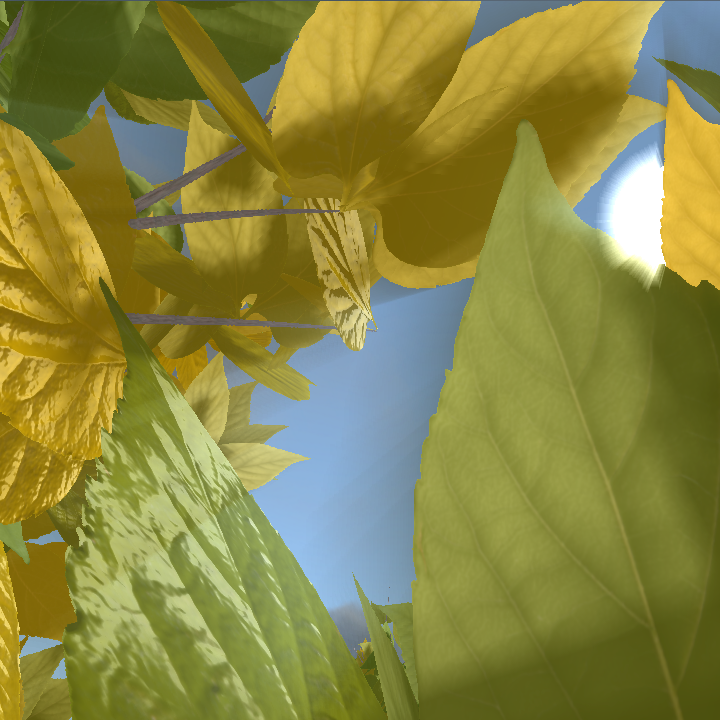
\includegraphics[width=0.45\textwidth]{./figures/final-leaves_H.png}&
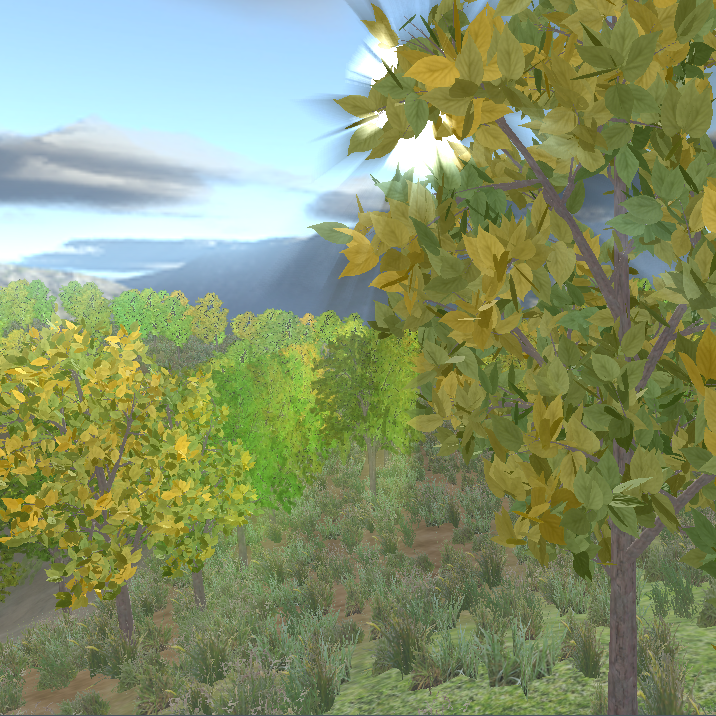
\includegraphics[width=0.45\textwidth]{./figures/final-trees_H.png}\\
(a)&(b)\\
\end{array}$
\caption[Ukázka výsledného zobrazení]%
{Výsledné zobrazení. Detail listů (a), kde je patrná průsvitnost i lesklost. Rozsáhlejší scéna s více stromy (b).\label{fig:resultA}
}
\end{center}
\end{figure}
V následujícím textu bude stručně popsáno, jejich řešení. Budou zmíněny technologie a knihovny, které byly pro realizaci použity, a popsána vstupní data výsledného programu, jejich zpracování a použití. Opomenuta nezůstane ani celková architektura systému a konkrétní řešení zobrazování všech úrovní detailu (LOD).

\pagebreak

%%%%%%%%%%%%%%%%%%%%%%%%%%%%%%%%%%%%%%%%%
\section{Použité technologie, frameworky a knihovny}
\label{sec-frameworks}

Výsledná aplikace byla implementována v jazyce {\bf C/C++} a využívá knihovnu {\bf OpenGL} \cite{openGL}. Ta poskytuje efektivní aparát pro práci s grafickým hardware a umožňuje využít většiny jeho nejnovějších vlastností a funkcí. Její výhodou je platformová nezávislost. Stejný kód by tedy mělo být možné přeložit jak pro Windows, tak pro systémy Unixového typu. Následně bylo využito několika dalších knihoven zjednodušujících práci se základní OpenGL:
\begin{description}
\item[GLFW] \cite{GLFW} sada knihovních funkcí určených pro snadné vytváření oken, OpenGL kontextů a mapování vstupních zařízení. Zachovává platformní nezávislost a uplatňuje se zejména ve fázi inicializace aplikace. Pomocí této knihovny je vytvořeno okno potřebných vlastností (podporuje i multisampling).
\item[GLUT] \cite{GLUT} sada nástrojů pro efektivnější práci. Obsahuje funkce pro vytváření oken a kontextů, mapování vstupů i pro práci s grafickými prvky.
\item[GLEW] \cite{GLEW} knihovna pro práci s rozšířeními (extenzemi) OpenGL. Zahrnuje zejména funkce pro zjišťování, zda ovladač grafického hardware danou extenzi podporuje.
\end{description}
Další knihovnou, která byla využita, je {\bf LODEpng} \cite{LODEpng}. Jde o jednoduchý dekodér a enkodér obrazového formátu PNG, který je distribuován formou jednoho \emph{.cpp} a jednoho {.h} souboru. Je s výhodou využit pro načítání obrázků do textur.

% obrázky zákl. ovládacích prvků
\begin{figure}[!hbt]
\begin{center}
$\begin{array}{cc}
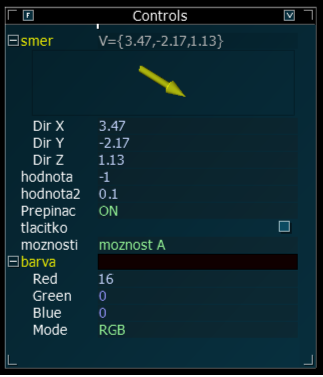
\includegraphics[width=0.35\textwidth]{./figures/ATWgui.png}&
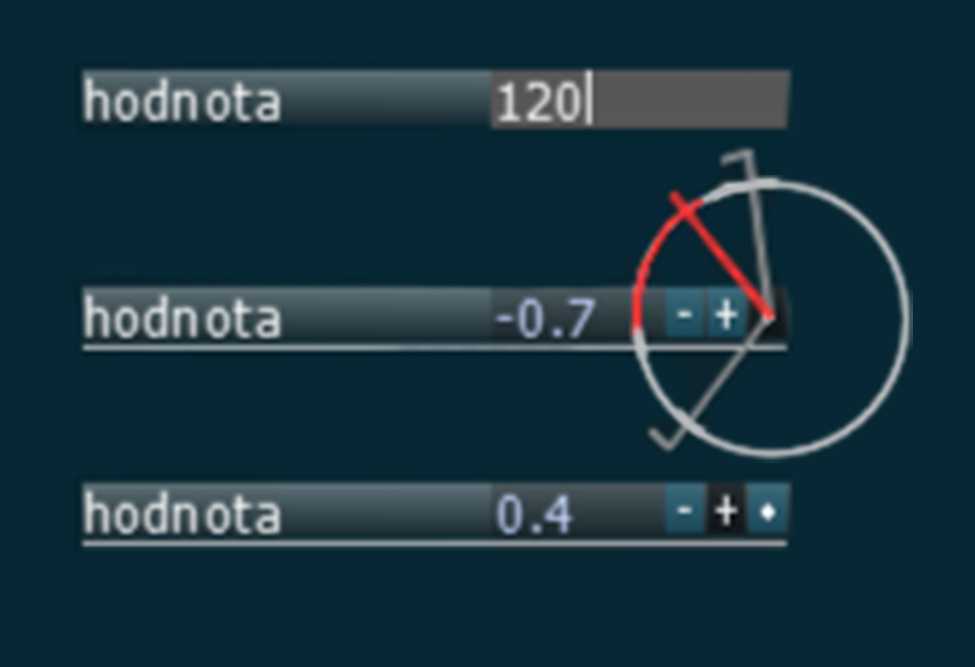
\includegraphics[width=0.3\textwidth]{./figures/ATWgui3.png}\\
(a)&(b)\\
\end{array}$
\caption[AntTweakBar, jednoduché GUI]%
{AntTweakBar, (a) ukázka základních ovládacích prvků (shora): ovladač směru, celočíselná skalární hodnota, desetinná skalární hodnota, dvoustavový přepínač, tlačítko, seznam možností, výběr barvy.  (b) různé způsoby zadávání hodnot (shora): přímé zadání, zadání pomocí tzv. RotoSlideru, pomocí krokovacích tlačítek \label{fig:ATWgui}
}
\end{center}
\end{figure}
Pro snadnou tvorbu grafického uživatelského rozhraní (dále jen GUI) byla využita knihovna {\bf AntTweakBar} \cite{AntTweakBar}. Ta umožňuje jednoduchou tvorbu grafických ovládacích prvků, které se nejčastěji používají při práci s 3D grafickou aplikací (viz obr. \ref{fig:ATWgui}). Těmito ovládacími prvky pak lze snadno bezprostředně a přímo ovlivňovat chování zobrazované scény - v tomto případě stromů.







%%%%%%%%%%%%%%%%%%%%%%%%%%%%%%%%%%%%%%%%%
\section{Architektura LOD}
\label{sec-LODarchitecture}
Realizace systému vykreslování a řízení úrovní jednotlivých stromů reflektuje možnosti současných grafických karet. Jelikož je objem dat zpracovávaný v každém snímku relativně velký a současně se z velké části nemění, lze tyto neměnná data přesunout do paměti GPU a tím i zefektivnit jejich zpracování. Ušetří se tím zbytečné přenosy po sběrnici mezi hlavní pamětí a pamětí grafické karty. Tento přístup je v dnešní době standardem a OpenGL ho samozřejmě podporuje ve formě tzv. \emph{Vertex Buffer Objects} (VBO), což je struktura obsahující data příslušná vrcholům jako jejich atributy (např.: pozice, normála, barva, atd.). 

\begin{figure}[!hbt]
\begin{center}
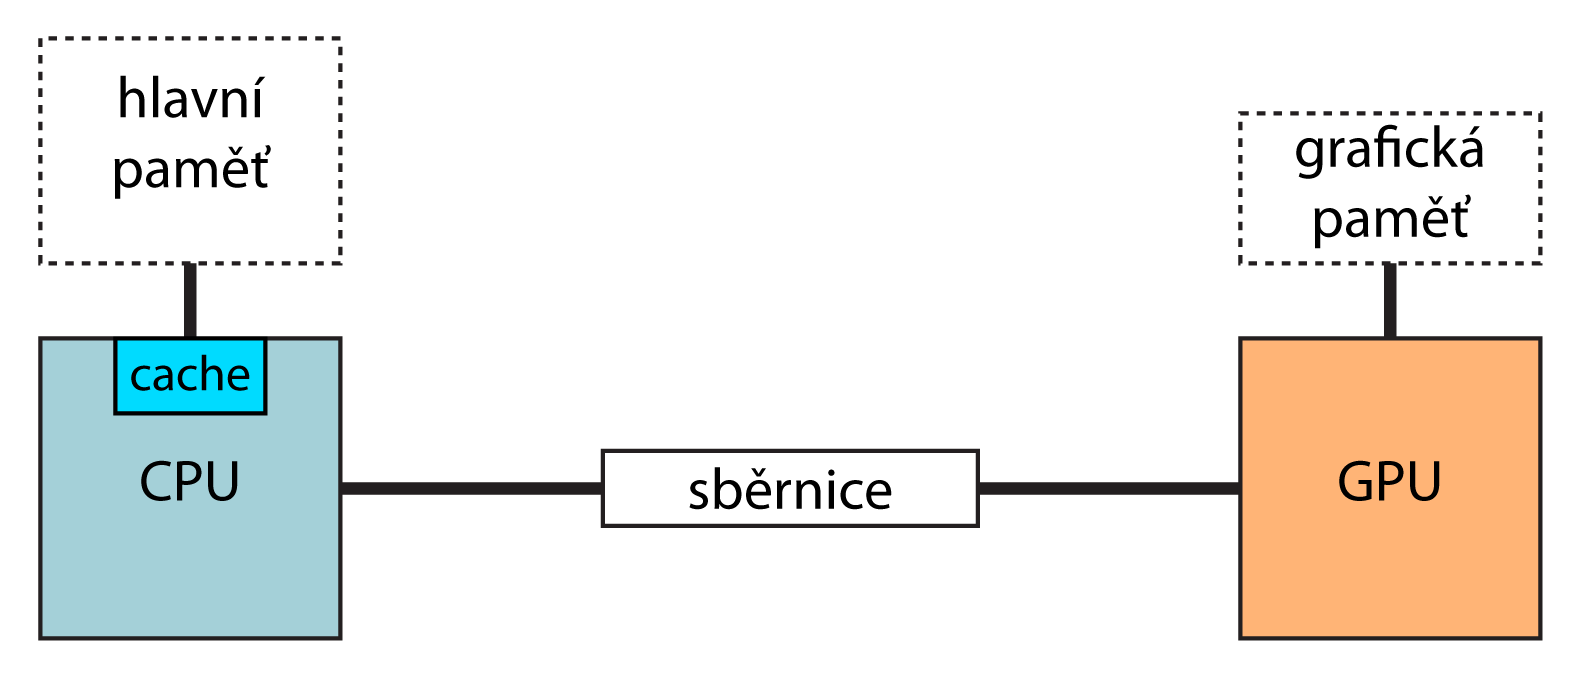
\includegraphics[width=0.75\textwidth]{./figures/CPUaGPU.png}
\end{center}
\caption[Různé druhy pamětí]%
{Různé druhy pamětí: hlavní paměť při CPU a grafická paměť na GPU. Přenos dat po sběrnici může mít negativní vliv na výkon.
\label{fig:CPUaGPU}
}
\end{figure}

Tato data mohou být umístěna jak v hlavní paměti, tak i v paměti GPU. Požadavek na umístění těchto dat lze vyjádřit při jejich zápisu do VBO příkazem 
\begin{verbatim}glBufferData(..., const GLvoid *  data, GLenum  usage)\end{verbatim}
Parametr \lineCode{usage} definuje povahu dat. Např. hodnota \lineCode{GL\_STATIC\_DRAW} informuje OpenGL o tom, že data se nebudou měnit a je tedy vhodné přesunout je do paměti GPU . Podle konkrétní implementace OpenGL a možností grafického hardware je tedy tedy tento přesun proveden, či je umístění dat jinak optimalizováno. Naproti tomu hodnota \lineCode{GL\_STREAM\_DRAW} naznačuje, že data budou v každém snímku změněna a přenos mezi CPU a GPU nelze ušetřit. Proto budou v takovém případě data raději v hlavní paměti.

Kromě VBO existuje ještě obdobný konstrukt pro uložení indexů indexované geometrie - tzv. \emph{Element Buffer Objects} (EBO). Indexovaná geometrie je výhodná zejména v případě, že se atributy vrcholů nemění a vrcholy jsou použity v rámci tvorby geometrie vícekrát (např. vrchol je společný pro mnoho trojúhelníků)

Protože se předpokládá zobrazení více instancí téhož stromu, jeví se jako přirozené využít techniky \emph{instancování na GPU}, která vytváří jednotlivé instance dynamicky až v rámci hardwaru. Tato technika se vyplácí zejména pro zpracování a zobrazování většího počtu instancí. Jeví se tedy jako vhodné, využít ji pro zobrazování zejména instancí s nižším LOD (LOD1 a LOD2), kterých je typicky řádově více než instancí nejvyššího detailu. Myšlenka instancování na GPU je prostá. Pokud se instance vzájemně liší pouze několika globálními parametry (pozice a orientace ve scéně, příp. další atributy) není třeba každou instanci vykreslovat zvláštním příkazem. Místo toho je typicky využit příkaz:
\begin{verbatim}glDrawElementsInstanced(..., GLsizei pocetInstanci)\end{verbatim}
Ten vykreslí zadaný počet instancí připojené indexované geometrie. Jelikož je však třeba jednotlivé instance správně umístit do scény a přiřadit jim i další specifické parametry, je třeba předat konkrétní instanci příslušná data. K tomu účelu se využívá princip tzv. \emph{instančních atributů}. Narozdíl od běžných atributů, které přísluší jednotlivým vrcholům (typicky normála, tangenta, texturovací souřadnice apod.), instanční atributy jsou stejné pro všechny vrcholy dané instance, ale liší se mezi instancemi. Toto chování lze zajistit příkazem:
\begin{verbatim}glVertexAttribDivisor(GLuint attribDesc, GLuint divisor)\end{verbatim}
Parametr \lineCode{divisor} určuje, pro kolik instancí bude atribut popsaný \lineCode{attribDesc} stejný. Hodnota $0$ vrací chování zpět na standardní - tedy atributy se různí pro jednotlivé vrcholy.
Instanční atributy je dobré uložit taktéž do VBO. Jelikož implicitně se všechny instance vykreslí díky použití stejných dat na stejnou pozici ve scéně, je nutné ve vertex shaderu transformovat všechny vrcholy dané instance příslušným způsobem. Z toho důvodu se jako jeden z instančních atributů předává i instanční transformační matice. Pořadí, v jakém jsou předány instanční atributy, určuje i pořadí vykreslování jednotlivých instancí.

Pro realizaci aplikace pracující s LOD jsou výše zmíněné možnosti zásadní. Jelikož je nutné v každém snímku určit pro každou instanci v jakém LOD se bude vykreslovat a to závisí v tomto případě na vzdálenosti od pozorovatele, jsou instance zpracovávány postupně a jsou přiřazeny do jedné ze zobrazovacích front (viz obr. \ref{fig:InstanceQueues}). 
\begin{figure}[!hbt]
\begin{center}
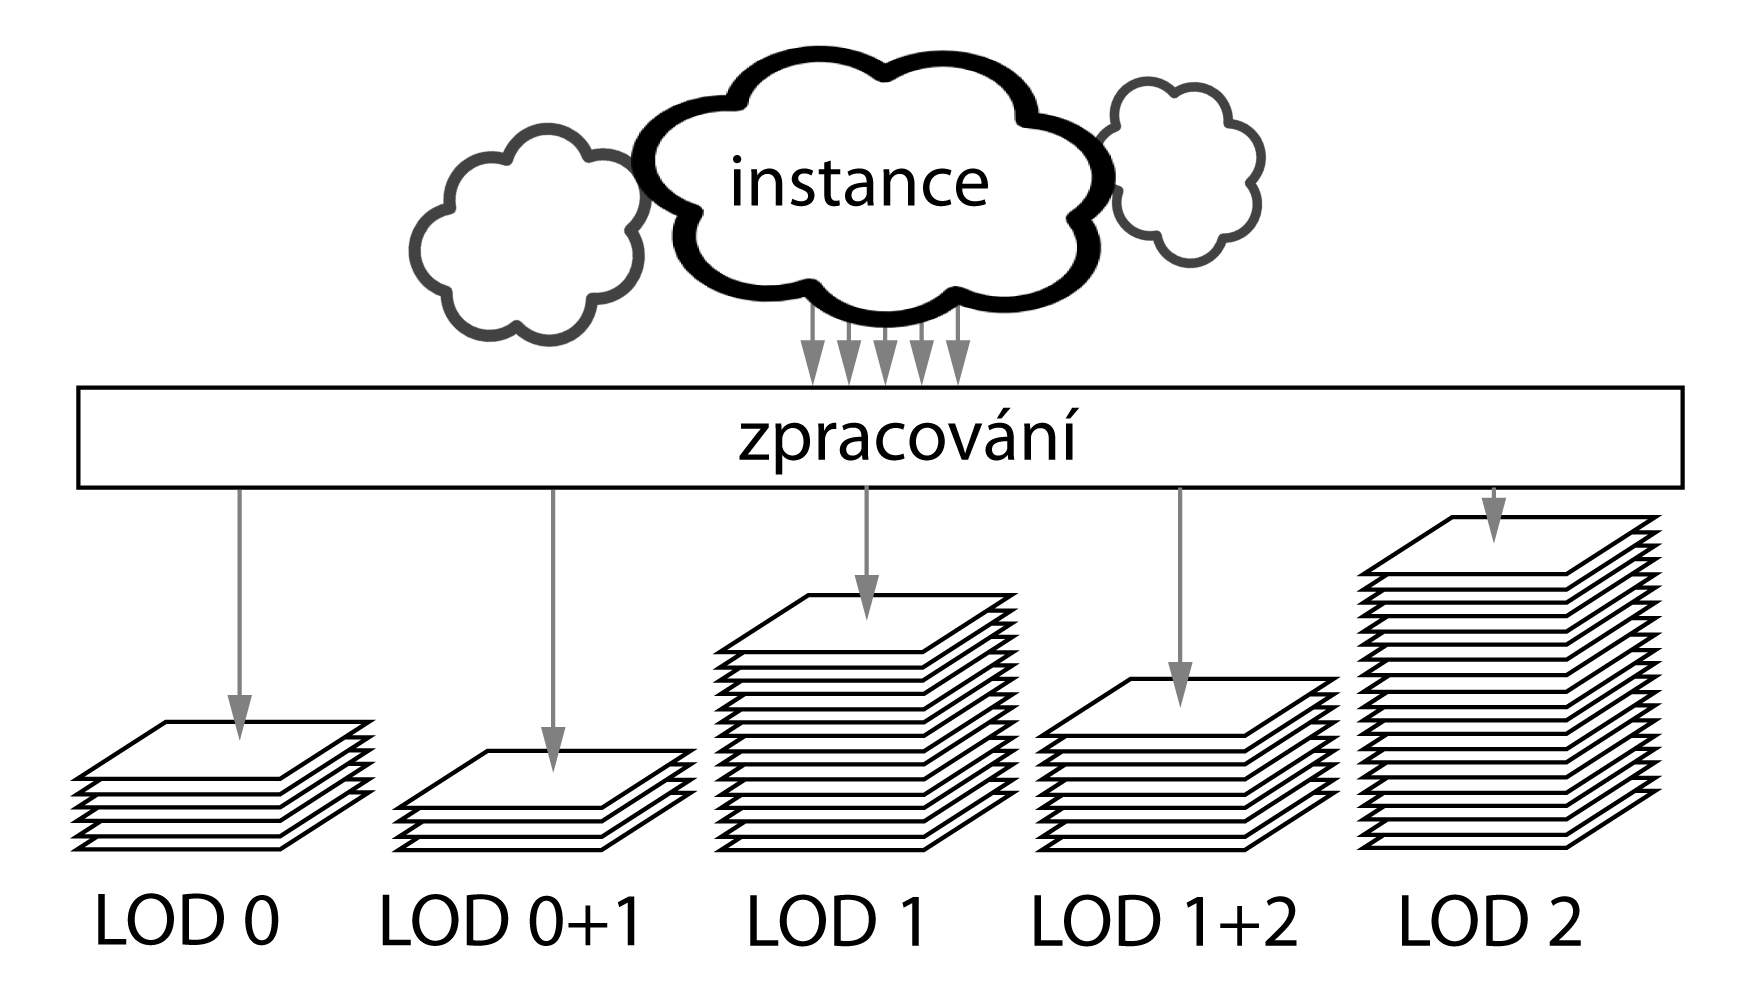
\includegraphics[width=0.5\textwidth]{./figures/renderQueuesA.png}
\end{center}
\caption[Fronty instancí]%
{Fronty instancí. LOD0 jsou instance v nejvyšším stupni detailu. Fronta LOD0+1 představuje instance v přechodu mezi úrovněmi LOD0 a LOD1. Obdobně i pro LOD2.
\label{fig:InstanceQueues}
}
\end{figure}
Některé instance pak lze vyřadit ze zobrazovacího procesu třeba proto, že neleží v prostoru aktuálního pohledu\footnote{stromy v těsném okolí pozorovatele ale mohou vrhat stín, a proto jsou zachovány} (např. leží za pozorovatelem). 

Instancím, které jsou pro daný pohled právě v přechodu mezi různými stupni LOD, je v rámci zpracování určena fáze přechodu a podle \cite{GIEGL-2007-UNP} jsou zobrazeny. V pseudokódu lze tento proces popsat následujícím způsobem:
\begin{verbatimtab}[4]
function makeTransition(float phase, Tree instance){
	float alpha1;
	float alpha2;
	if (phase<0.5){
		alpha1 = 1;	
		alpha2 = 2*phase;
		disableDepthBufferWrite();
			instance.drawLOD_B(instance, alpha2);
		enableDepthBufferWrite();
		instance.drawLOD_A(instance, alpha1);					
	} else {			
		alpha1 = 2*(1-phase);
		alpha2 = 1;	
		instance.drawLOD_B(instance, alpha2);	
		disableDepthBufferWrite();
			instance.drawLOD_A(instance, alpha1);
		enableDepthBufferWrite();	
	} 
}
\end{verbatimtab}

Kvůli průhlednosti, která hraje důležitou roli u nižších úrovní detailu, a která není implicitně řešena v rámci OpenGL, je nutné provádět vykreslování v pořadí od vzdálených instancí k bližším. Z toho důvodu je třeba provádět v rámci zpracování rychlé řazení instancí před vykreslením každého snímku \footnote{předpokládáme-li změnu pozice a pohledu pozorovatele}. Důležitý je fakt, že mezi následujícími snímky je zachována určitá koherence. Instance, které jsou v seřazeném pořadí v jednom snímku blízko sebe, budou nejspíš kdesi blízko sebe i ve snímku následujícím. S výhodou tedy lze použít částečného řazení s nižší (lineární) časovou složitostí. V tomto případě je využito jednoho průchodu algoritmu známého jako \emph{bubble-sort} (dále jen \emph{lazy-sort} neboli \emph{líné řazení}). Toto řazení funguje na úrovni jednotlivých instancí a poskytuje uspokojivé výsledky. 
Fronty instancí LOD1 a LOD2 jsou následně vykreslovány pomocí instančního zobrazování. Ostatní fronty, u kterých se předpokládá, že neobsahují tolik položek, jsou vykreslovány po jednotlivých instancích.


%%%%%%%%%%%%%%%%%%%%%%%%%%%%%%%%%%%%%%%%%
\section{Vstupní data a předzpracování}
\label{sec-modelAnalysis}
Aplikace načítá celou řadu dat, se kterými dále pracuje. V první řadě je nutné načíst popis stromu, dále pak textury použité pro jeho zobrazení. Načtená data je v řadě případů nutno předzpracovat, aby je bylo možné využít. Právě popisem vstupních dat a jejich předzpracováním se bude zabývat následující text.

%%%%%%%%%%%%%%%%%%%%%%%%%%%%%%%%%%%%%%%%%%%
\subsection{Formát OBJT}
Jelikož běžné modely stromů neobsahují implicitně informace o topologii stromu, která je nezbytná pro provedení animace, byl navržen formát vstupního souboru OBJT, který zahrnuje právě tyto informace. Soubor formátu OBJT je vstupním souborem popisujícím model stromu. OBJT je textový formát obsahující 4 druhy záznamů (oddělených standardním oddělovačem řádků):
\begin{itemize}
\item pojmenování stromu na začátku souboru entitou \lineCode{name = "\%sting\%"}
\item entita popisující větev \begin{verbatimtab}
B  %int% { 			// identifikátor větve
  l   	%int%			// úroveň v hierarchii
  d 	%float%			// délka větve
  z  	%float%	%float%	%float%	// pozice začátku větve
  k 	%float%	%float%	%float%	// pozice konce větve
  r  	%float%	%float%	%float%	// bázový vektor r
  s  	%float%	%float%	%float%	// bázový vektor s
  t  	%float%	%float%	%float%	// bázový vektor t (podélný)
  p  	%int%			// identifikátor rodičovské větve
  x  	%float%	// v kolikátině rodičovské větve se větev odpojuje
}
\end{verbatimtab}
\item entita popisující list  \begin{verbatimtab}
L  %int% { 			// identifikátor listu
  r  	%float%	%float%	%float%	// bázový vektor r
  s  	%float%	%float%	%float%	// bázový vektor s
  t  	%float%	%float%	%float%	// bázový vektor t (podélný)
  p  	%int%			// identifikátor rodičovské větve
  x  	%float%	// v kolikátině rodičovské větve se list odpojuje
}
\end{verbatimtab}
\item řádkový komentář začínající \lineCode{// \%string\%}
\end{itemize}

Ve výše uvedeném popisu formátu jsou použity zástupné řetězce za celá čísla (\lineCode{\%int\%}), za desetinná čísla (\lineCode{\%float\%}) a za znakové řetězce bez oddělovače konce řádků (\lineCode{\%string\%}). Všechny souřadnice se předpokládají v souřadném systému celého stromu (též \emph{object space}).

Data ze zdrojového OBJT jsou načtena, větve jsou vytvořeny jako kužely a listy jako ploché čtverce (quads). Vrcholy a jejich atributy jsou následně uloženy do VBO. Těmito daty jsou:
\begin{itemize}
\item pozice v souřadném systému větve
\item normála a tangenta v souřadném systému rodičovské větve
\item texturovací souřadnice
\item vektor hodnot x (viz obr.~\ref{fig:hierarchyCoords})
\item souřadnice do datové textury pro příslušnou větev (její obsah bude popsán dále)
\end{itemize}

%%%%%%%%%%%%%%%%%%%%%%%%%%%%%%%%%%%%%%%%%%%
\subsection{Textury}
\label{sec:Textury}
Ačkoliv je v celé aplikaci použito velké množství textur (pro skybox, krajina, atd.), zde budou zmíněny pouze ty nejdůležitější, které se vážou přímo k tématu zobrazování stromů.

Pro zobrazení 3D modelu stromu je použito několik textur, které jsou načítány při spuštení aplikace. Kromě textur použitých pro zobrazení listů (viz obr.~\ref{fig:leafResources}) je pro obarvení kmene a větví načtena textura jejich struktury (viz obr.~\ref{fig:branchResources}).
\begin{figure}[!hbt]
\begin{center}
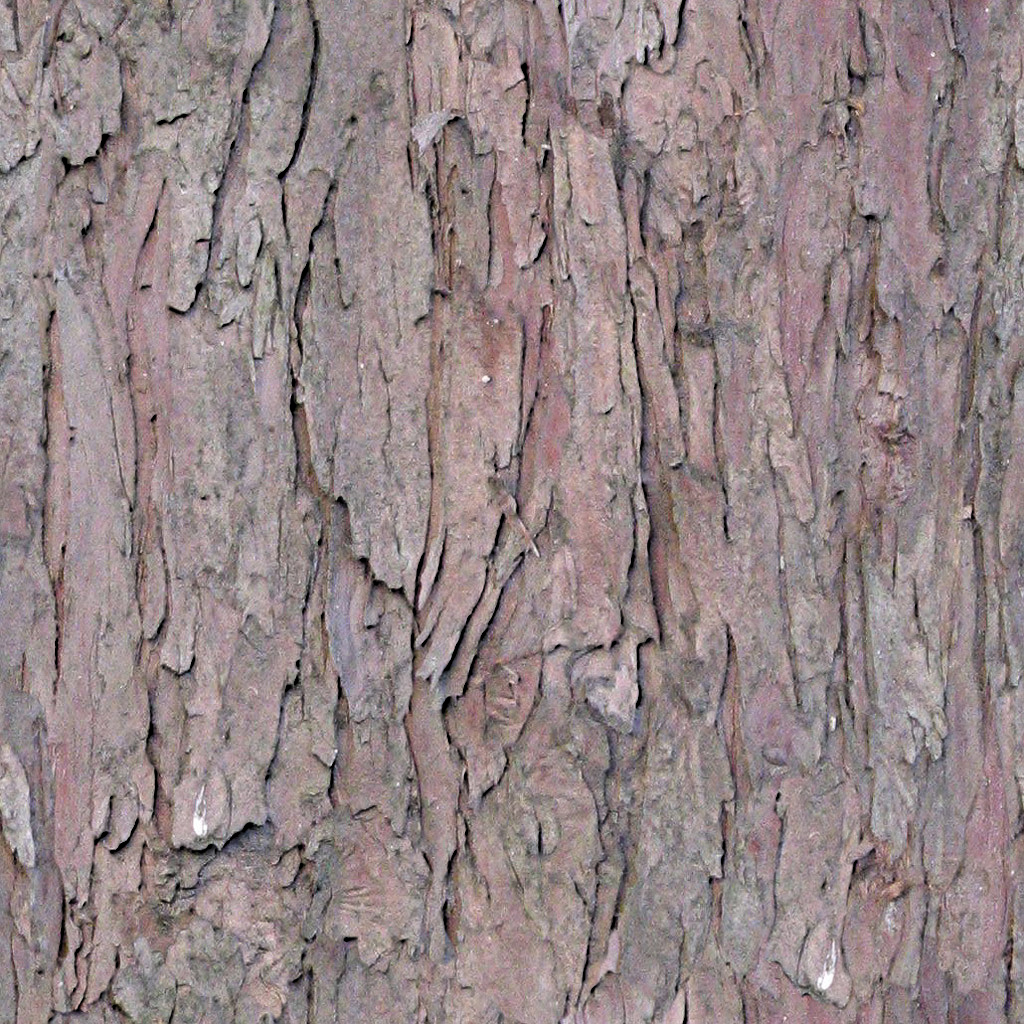
\includegraphics[width=0.35\textwidth]{./figures/bark2_decal.png}
\end{center}
\caption[Zdrojová textura barvy kmene a větví]%
{Zdrojová textura barvy kmene a větví. \label{fig:branchResources}
}
\end{figure}

Dále jsou načteny šumové textury řídící animaci (obr.~\ref{fig:noiseResources})
\begin{figure}[!hbt]
\begin{center}
$\begin{array}{cc}

\includegraphics[width=0.4\textwidth]{./figures/branch_noise.png}&

\includegraphics[width=0.4\textwidth]{./figures/leaf_noise.png}\\
(a)&(b)
\end{array}$
\end{center}
\caption[Šumové textury animace větví a listů]%
{Šumové textury animace větví (a) a listů (b) \label{fig:noiseResources}
}
\end{figure}

Přímo zásadní je však textura, v níž jsou uložena data potřebná pro provedení deformace ve vertexovém procesoru. Tuto texturu je nutné pro daná vstupní data popisující strom vytvořit.
Pro její sestavení je třeba převést zejména bázové vektory větve ($\vec{r}$, $\vec{s}$, $\vec{t}$) do souřadného systému rodičovské větve (převedené vektory $\vec{r_b}$, $\vec{s_b}$, $\vec{t_b}$). Zároveň je potřeba pro každou větev vytvořit (pokud možno) unikátní vektor $\vec{mv}$ posunu v šumové textuře. Informace doplňují záznamy o délkách rodičovských větví $l_0-3$. Jelikož je třeba uložit do textury normalizované vektory, je použita textura typu \lineCode{GL\_RGBA32F}. 

Minimální sada dat v datové textuře tedy vypadá následovně:
\begin{table}[!hbt]
\catcode`\-=12
\begin{center}
\begin{tabular}{c | c | c | c | c | c | c | c | c | c | c |} 
 & \multicolumn{10}{c}{obsah textury}\\
i+1 & \multicolumn{10}{c |}{\vdots}\\
\cline{1-11}
\multirow{4}{*}{i} & $\vec{mv_0}.x$ 	& $\vec{mv_2}.x$ 	&  $\vec{s_{b,0}}.x$  & $\vec{s_{b,1}}.x$  & $\vec{s_{b,2}}.x$  & $\vec{s_{b,3}}.x$  & $\vec{r_{b,0}}.x$  & $\vec{r_{b,1}}.x$  & $\vec{r_{b,2}}.x$  & $\vec{r_{b,3}}.x$\\
\cline{2-11}
& $\vec{mv_0}.y$ 		& $\vec{mv_2}.y$ 	&  $\vec{s_{b,0}}.y$  & $\vec{s_{b,1}}.y$  & $\vec{s_{b,2}}.y$  & $\vec{s_{b,3}}.y$  & $\vec{r_{b,0}}.y$  & $\vec{r_{b,1}}.y$  & $\vec{r_{b,2}}.y$  & $\vec{r_{b,3}}.y$\\
\cline{2-11}
& $\vec{mv_1}.x$ 		& $\vec{mv_3}.x$  	&  $\vec{s_{b,0}}.z$  & $\vec{s_{b,1}}.z$  & $\vec{s_{b,2}}.z$  & $\vec{s_{b,3}}.z$  & $\vec{r_{b,0}}.z$  & $\vec{r_{b,1}}.z$  & $\vec{r_{b,2}}.z$  & $\vec{r_{b,3}}.z$\\
\cline{2-11}
& $\vec{mv_1}.y$ 		& $\vec{mv_3}.y$ 	&  $l_0$  &$l_1$  & $l_2$ & $l_3$  &  & & & \\
\hline
i-1 & \multicolumn{10}{c |}{\vdots}\\
\end{tabular}
\label{table:dataTexture}
\caption{Minimální sada dat uložená v datové textuře pro LOD0.}
\end{center}
\end{table}

\begin{figure}[!hbt]
\begin{center}

\includegraphics[width=0.05\textwidth]{./figures/branchDataTextureLOD0.png}
\end{center}
\caption[Ukázka z datové textury pro LOD0]%
{Ukázka z datové textury pro LOD0. Číslo řádku $i$ odpovídá identifikátoru větve.\label{fig:branchDataTextureLOD0}
}
\end{figure}
Velice důležitou je textura sezónních barev (viz obr. ~\ref{fig:seasonMap}). Jde o jednořádkovou texturu. Z ní je interpolována sezónní barva ve smyslu členu $c_s(s)$ ze vztahů \eqref{eq:color_def}. Parametr \lineCode{sezona} lze použít přímo jako souřadnici do této textury. 
\begin{figure}[!hbt]
\begin{center}

\includegraphics[width=0.6\textwidth]{./figures/seasonTex.png}
\end{center}
\caption[Ukázka textury sezónních barev]%
{Ukázka textury sezónních barev. Obrázek je zvětšený, otočený o $90^{\circ}$ a šedá šachovnice vizualizuje průhledné pixely.\label{fig:seasonMap}
}
\end{figure}

Zobrazování LOD1 a LOD2 vyžaduje rovněž vytvoření několika speciálních textur. Jejich vytvořením se zabývá další sekce (\ref{sec:preprocessLOD}).

\pagebreak
%%%%%%%%%%%%%%%%%%%%%%%%%%%%%%%%%%%%%%%%%%%
\subsection{Předzpracování pro LOD}
\label{sec:preprocessLOD}
Pro zobrazení a animaci LOD1 a LOD2 je třeba vytvořit během předzpracování sadu textur. Jednak je to množina textur, které jsou nezbytné i pro zobrazení statického stromu, druhak se pak přidávají i textury, jež jsou nezbytné pro provedení animace. Následující popis uvádí postup generování těchto textur pro LOD1. Pro LOD2 je postup obdobný.

Ke zobrazení statického stromu pomocí trsu řezů je třeba vytvořit textury obsahující pohled na strom z daného úhlu v několika vrstvách. Tyto textury lze relativně jednoduše generovat použitím techniky \emph{offscreen-rendering} neboli vykreslování do textur. V OpenGL se toho dosáhne připojením speciálního tzv. \emph{Frame Buffer Object} (FBO) s napojenými texturami (viz obr.~\ref{fig:FBO}).
\begin{figure}[!hbt]
\begin{center}
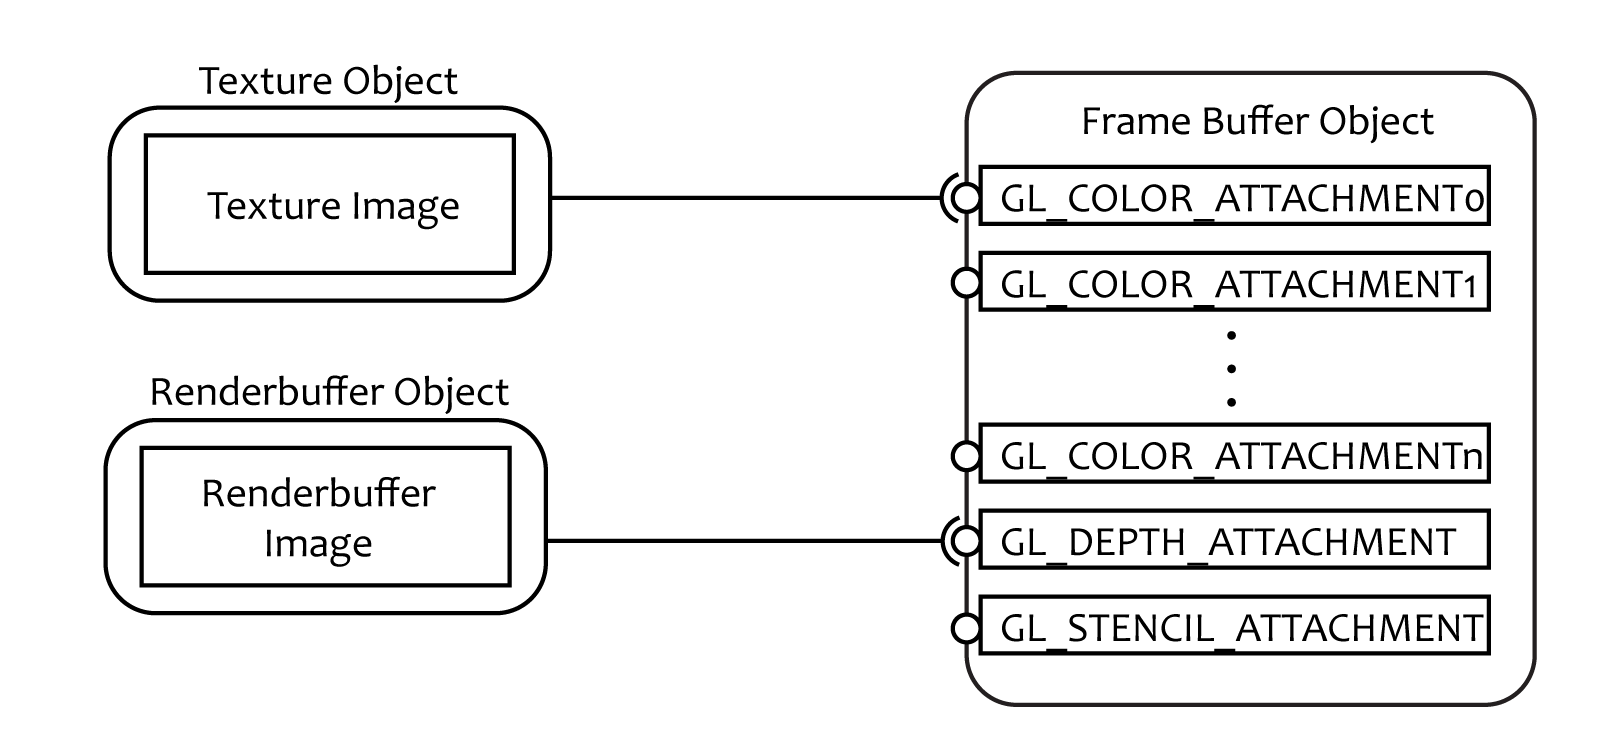
\includegraphics[width=0.7\textwidth]{./figures/FBO.png}
\end{center}
\caption[Mechanismus FBO v OpenGL]%
{Mechanismus Frame Buffer Object v OpenGL.\label{fig:FBO}
}
\end{figure}


 Následující kód ukazuje, jak takovýto FBO vytvořit:
\begin{alltt}
\textit{// vytvoreni FBO}
GLuint	fboID = 0;
GLenum buffers[3] = \{ GL_COLOR_ATTACHMENT0,
                      GL_COLOR_ATTACHMENT1,
                      GL_COLOR_ATTACHMENT2 \};
glGenFramebuffers(1, &fboID);
glBindFramebuffer(GL_FRAMEBUFFER, fboID);
   glFramebufferTexture2D(GL_FRAMEBUFFER, GL_COLOR_ATTACHMENT0, GL_TEXTURE_2D,
                          colorTextureID, 0);
   glFramebufferTexture2D(GL_FRAMEBUFFER, GL_COLOR_ATTACHMENT1, GL_TEXTURE_2D,
                          normalTextureID, 0);
   glFramebufferTexture2D(GL_FRAMEBUFFER, GL_COLOR_ATTACHMENT2, GL_TEXTURE_2D, 
                          branchTextureID, 0);
   glFramebufferTexture2D(GL_FRAMEBUFFER, GL_DEPTH_ATTACHMENT, GL_TEXTURE_2D, 
                          depthTextureID, 0);
glBindFramebuffer(GL_FRAMEBUFFER, NULL);
\end{alltt}
\pagebreak
Použití - tedy přesměrování vykreslování do vytvořeného FBO probíhá následovně:
\begin{alltt}
\textit{// pouziti FBO}
{\bf setupCamera();}      \textit{// nastaveni kamery podle smeru a hloubky rezu}
glBindFramebuffer(GL_FRAMEBUFFER, fboID);
      glDrawBuffers(3, buffers);			
           {\bf draw();}     \textit{// vykresleni do pripojenych textur}
      glDrawBuffer(GL_BACK);
glBindFramebuffer(GL_FRAMEBUFFER, NULL);
\end{alltt}

Pro generování řezů je kamera nastavena na orthogonální projekci a vykreslení pouze určitého řezu je zajišteno správným nastavením přední a zadní ořezové roviny kamery ($near$, $far$). Jelikož se v této fázi vykresluje celý strom v normované jednotkové velikosti, je určení hodnot $near$ a $far$ triviální pro $i$-tý řez z daného směru : 
\begin{align}
thickness &= \frac {diameter_{tree}}{count_{slice}}\nonumber \\
near_i &= distance_{camera}-(0.5 \cdot diameter_{tree}) + i \cdot thickness \nonumber\\
far_i &= near_i + thickness
\end{align}

Nastavení projekční matice kamery zajišťuje funkce:
\begin{alltt}
glOrtho(float l, float r, float b, float t, float {\bf near}, float{\bf  far});
\end{alltt}

Pro každý řez je vytvořena následující sada textur:
\begin{itemize}
\item barevná textura
\item hloubková textura
\item normálová textura
\item textura větvových bodů
\end{itemize}

Do textur je vykreslen geometrický model v základní pozici (neovlivněný působením větru). Do barevné textury se zapíše nestínovaná barva bez sezónní složky, do textury normál se zapíše pro každý fragment normála (pouze 3 souřadnice) v souřadném systému řezu (budoucí \emph{tangent space}). Čtvrtá složka zaznamenává případně specifické číslo listu. Význam hloubkové mapy je zřejmý. Do textury větvových bodů se zaznamenávají identifikátory rodičovských větví 1. úrovně (napojené přímo na kmen). Následně je na této textuře provedena expanze dat (viz obr.~\ref{fig:dataExpansionExample}).
\pagebreak
%%%
% obrazek pred a po expanzi dat
%
\begin{figure}[!hbt]
\begin{center}
$\begin{array}{cc}
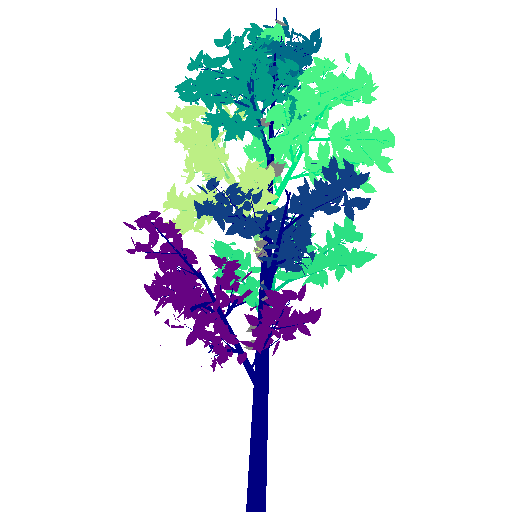
\includegraphics[width=0.30\textwidth]{./figures/dataPreExpanded.png}&
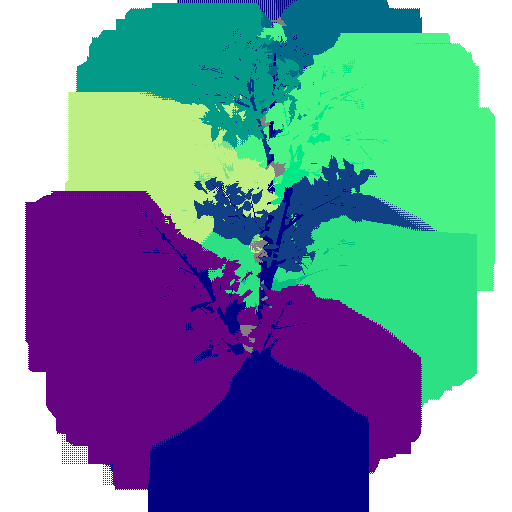
\includegraphics[width=0.30\textwidth]{./figures/dataExpanded.png}\\
(a)&(b)
\end{array}$
\end{center}
\caption[Ukázka expanze dat]%
{Ukázka expanze dat (změněna barevnost pro lepší zřetelnost). (a) před expanzí, (b) po expanzi.\label{fig:dataExpansionExample}
}
\end{figure}

Textury daného typu (barevné, normálové, \dots) jsou následně sloučeny dohromady (viz obr.~\ref{fig:joinTextures}). Děje se tak z důvodu ušetření texturovacích jednotek, jejichž počet je hardwarově omezen. Pro LOD1 s 3 směry řezů po 3 vrstvách a 4 sadami textur by tedy bylo nutné připojit $ (3 \times 3 \times 4 ) = 36 $ textur. Místo toho stačí připojit pouze 4 sloučené textury, což představuje značnou úsporu.
%%%
% obrazek pred a po expanzi dat
%
\begin{figure}[!hbt]
\begin{center}
\fbox{
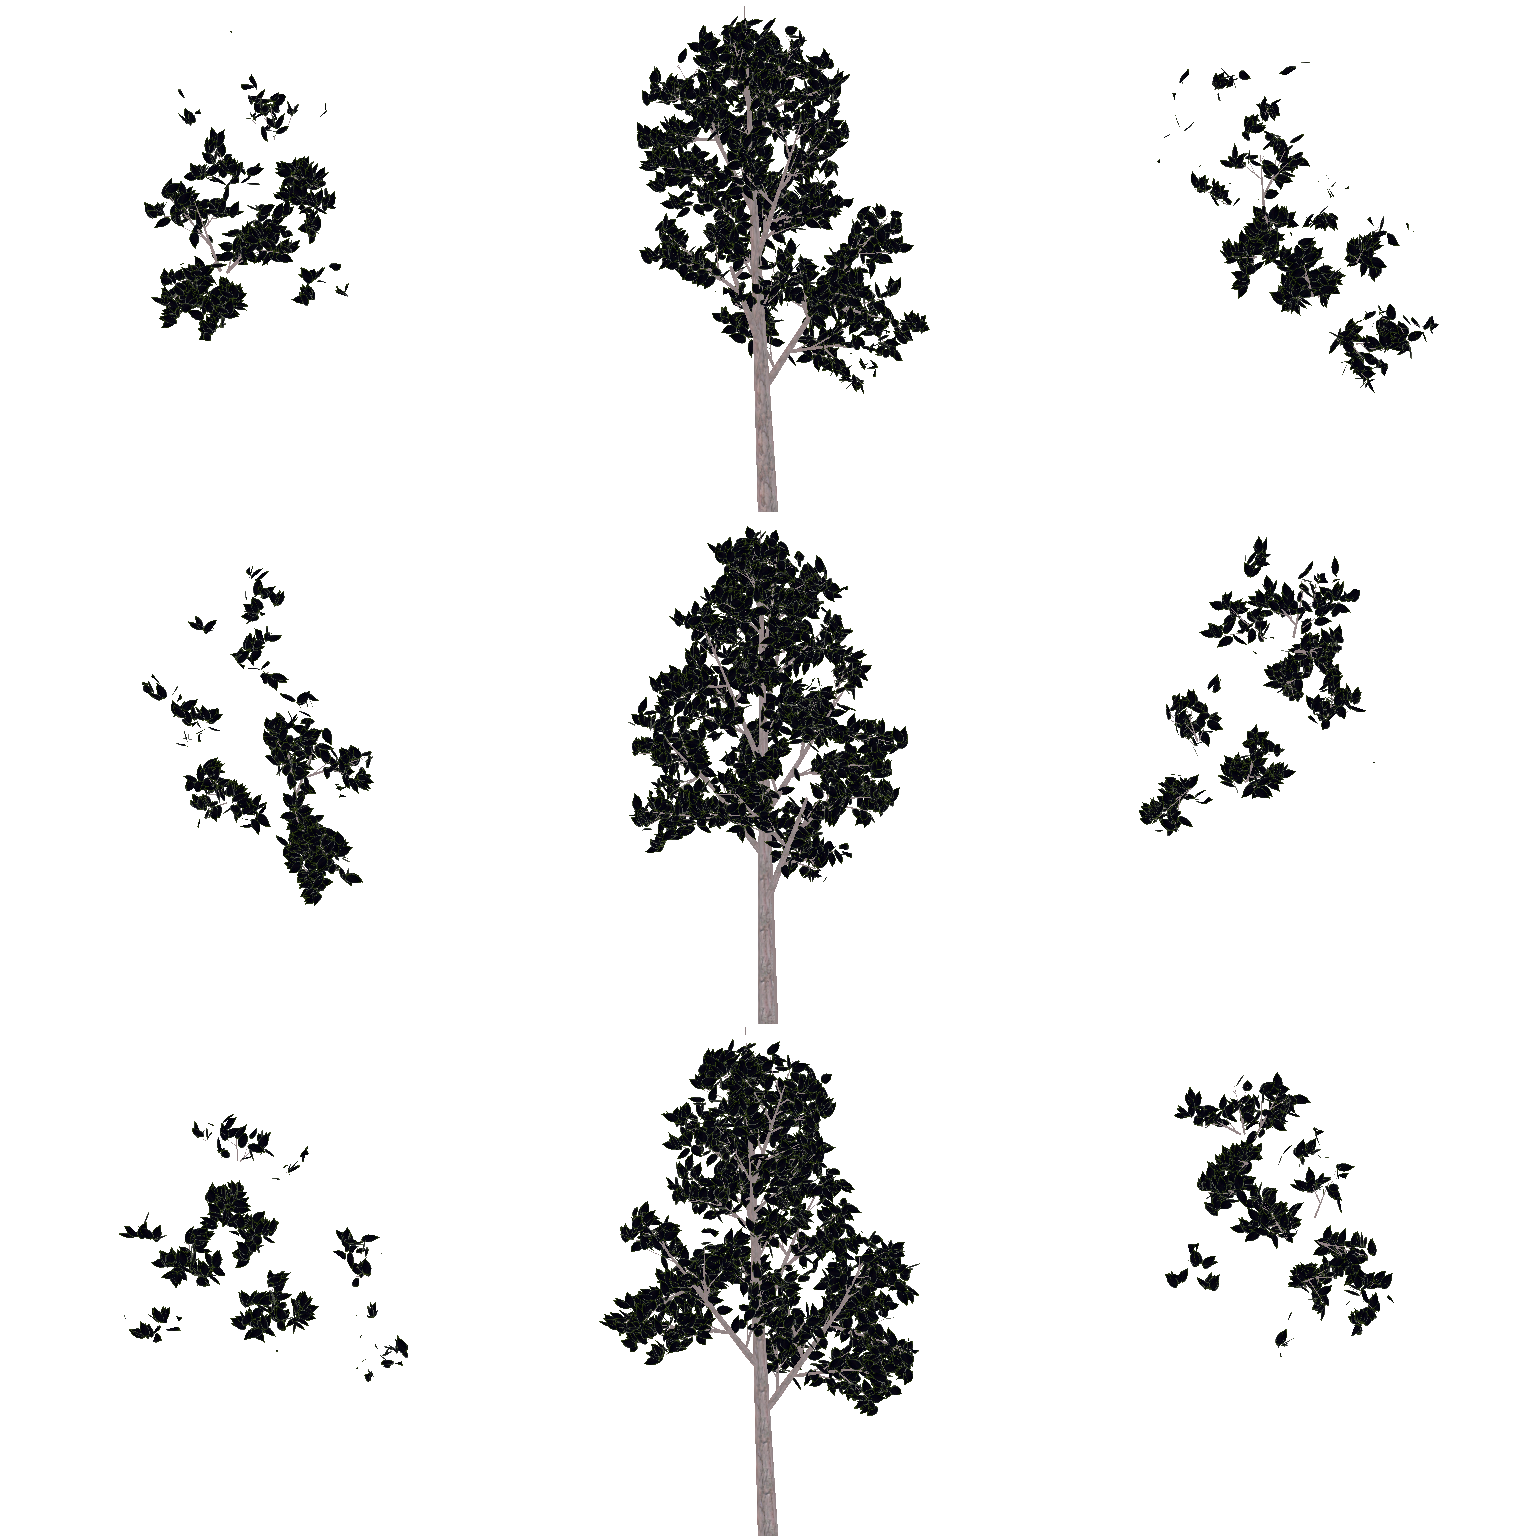
\includegraphics[width=0.4\textwidth]{./figures/joinTextures.png}
}
\end{center}
\caption[Slučování textur]%
{Slučování textur. Ukázka sloučení barevných textur pro LOD1 do jedné textury. .\label{fig:joinTextures}
}
\end{figure}

\pagebreak

Zásadní pro provádění animace v LOD operujícími nad trsy řezů je rovněž datová textura s informacemi o jednotlivých větvích. Tato textura obsahuje záznam pro každou větev, který obsahuje infromace o počátku větve v souřadném systému řezu, bázové vektory větve převedené rovněž do souřadného sytému řezu, projektovanou délku a pohybové vektory směru posunu v šumové textuře. Tyto informace se různí pro různé směry řezů a musí být tudíž zapsány i do textury pro každý směr zvlášť.


Data v datové textuře jsou tedy následující:
\begin{table}[!hbt]
\catcode`\-=12
\begin{center}
\begin{tabular}{c | c | c | c | c } 
 & \multicolumn{4}{c}{obsah textury}\\
 & \multicolumn{3}{c }{data řezu $j$} & data řezu $j+1$\\
$i+1$ & \multicolumn{3}{c |}{\vdots} & \vdots\\
\cline{1-5}
\multirow{4}{*}{$i$} 	& $\vec{o_s}.x$ 	& $\vec{r_s}.x$ 	&  $\vec{s_s}.x$ &  \multirow{4}{*}{\dots}\\
\cline{2-4}
				   	& $\vec{o_s}.y$ 	& $\vec{r_s}.y$  &  $\vec{s_s}.y$  & \\
\cline{2-4}
					& $\vec{mv}.x$ 	& $\vec{r_s}.z$  &  $\vec{s_s}.z$  & \\
\cline{2-4}
					& $\vec{mv}.y$  & $l_s$ 	&    & \\
\hline
$i-1$ & \multicolumn{3}{c |}{\vdots}&\vdots\\
\end{tabular}
\label{table:dataTexture}
\caption{Minimální sada dat uložená v datové textuře pro LOD1 a LOD2.}
\end{center}
\end{table}
\begin{figure}[!hbt]
\begin{center}

\includegraphics[width=0.05\textwidth]{./figures/branchDataTextureLOD1.png}
\end{center}
\caption[Ukázka části  datové textury pro LOD1]%
{Ukázka části datové textury pro LOD1. Číslo řádku $i$ odpovídá identifikátoru větve.\label{fig:branchDataTextureLOD1}
}
\end{figure}

%%%%%%%%%%%%%%%%%%%%%%%%%%%%%%%%%%%%%%%%%%%
\subsection{Dynamické parametry}
Aplikace nabízí možnost měnit dynamicky řadu parametrů souvisejících s animace stromů i s jejich zobrazováním. Nejpodstatnější jsou zejména tyto: \newline

\begin{tabular}{l} 
- směr větru\\
- síla větru\\
- amplituda větví (pro každou úroveň zvlášť)\\
- frekvence větví (pro každou úroveň zvlášť)\\
- amplituda listů\\
- frekvence listů\\
- prahy přechodů LOD\\
- sezóna\\
- směr světla\\
\end{tabular}



%%%%%%%%%%%%%%%%%%%%%%%%%%%%%%%%%%%%%%%%%
\section{Zobrazení geometrického modelu}
\label{sec-3Ddisplay}
Vykreslování stromu v nejvyšší úrovni detailu probíhá v souladu s teorií popsanou v kapitole~\ref{chap:analyza}. Vykreslování probíhá ve 2 fázích, nejprve se vykreslí kmen a větve, poté jednotlivé listy. V každé z těchto fází je aktivní jiný shader (program řídící částečně činnost GPU).

%%%
% vetve
%
 Jednotlivé větve jsou zobrazovány jako kužely různých délek a průměrů. Jednotlivé vrcholy tvořící větev jsou zadané v souřadném systému příslušné větve. Dalšími atributy větvových vrcholů jsou: normála, tangenta, texturovací souřadnice, index větve v datové textuře a vektor hodnot $x$ (hierarchické souřadnice viz obr. ~\ref{fig:hierarchyCoords} ). Parametry ohybové funkce $c_2$ a $c_4$ (viz ~\ref{eq:bendFunction}) byly zafixovány na hodnotách $c_2 = 0.374570$ a $c_4 = 0.129428$, což odpovídá hodnotě parametru $\alpha = 0.2$ (viz~\ref{eq:EulerBernoulliFunction})
 Nejdůležitější část kódu vertex shaderu je schematicky popsaná níže:
\begin{nobreak}  
\begin{alltt}
\textit{// center \dots pozice stredoveho ridiciho bodu}
\textit{// t \dots podelny vektor}
\textit{// r \dots kolmy vektor, normala}
\textit{// s \dots kolmy vektor, binormala}
\textit{// x \dots hierarchicka souradnice}
\textit{// amp \dots ridici signal animace}
\textit{// length \dots delka vetve}
void{\bf bend}(inout vec3 center, inout vec3 t, inout vec3 r, inout vec3 s,
          in float x, in vec2 amp, in float length)\{
  float fx = 0.374570*x*x + 0.129428*x*x*x*x;
  float dx = 0.749141*x + 0.517713*x*x*x;
  vec3 corr_r = vec3(0.0); vec3 corr_s = vec3(0.0);
\textit{// vychylkovy prispevek smerove slozky vetru }
  amp.x += dot(r, wind_direction) * wind_strength;
  amp.y += dot(s, wind_direction) * wind_strength;
\textit{// ohybova funkce }		
  fu	= fx	 * amp;
  fu_deriv = dx / length * amp ;
\textit{// zamezeni deleni nulou}
  fu_deriv = max(fu_deriv, EPSILON) + min(fu_deriv, EPSILON);
\textit{// korekce delky}		
  vec2 su = sqrt(vec2(1.0) + fu_deriv*fu_deriv);
  vec2 du = fu / fu_deriv * (su - vec2(1.0));
  corr_r = (t + r*fu_deriv.x)/su.x * du.x;
  corr_s = (t + s*fu_deriv.y)/su.y * du.y;
\textit{// ohnout stredovy bod a souradny system vetve}
  center =  center + x * length * t + fu.x * r + fu.y * s - (corr_s+corr_r);		
  t = normalize(t + r*fu_deriv.x + r*fu_deriv.y);
  r = normalize(r - t*fu_deriv.x);
  s = normalize(s - t*fu_deriv.y);	
\}\end{alltt}
\end{nobreak} 
\pagebreak
Následně se postupuje od úrovně 0 - tedy od kmene a provádí se ohyb pomocí popsané funkce {\bf bend}. Pro korektní ohyb je nutné deformovat (natočit) i souřadný systém následující úrovně větví. K tomu se využije skutečnosti, že báze jsou zadané v souřadném systému rodičovské větve. Stačí tedy provést triviální transformaci (br, bs, bt jsou ohnuté bázové vektory rodičovské větve):
\begin{alltt}
   s = s.x * br + s.y * bs + s.z * bt;
   r = r.x * br + r.y * bs + r.z * bt;
   t = cross( r , s );
\end{alltt}
Po provedení všech deformací v hierarchii získáme polohu bodu na středovém paprsku příslušné větve. Je tedy nutné ještě odsadit takový bod na povrch větve - využijeme proto vstupního atributu, který udává pozici bodu v souřadném systému větve:
 \begin{alltt}
  position = origin + position.x * br + position.y * bs;	
\end{alltt}

Při zobrazování listů se provede stejný postup deformací (list je spojený s větví a pohybuje se s ní), ovšem místo konečného odsazení se provede rotace souřadného systému animující pohyb listu.
 \begin{alltt}
  vec3 bitangent = cross( normal , tangent);
\textit{// natocit bazovy system listu}
  tangent = normalize ( tangent + normal * amplitude.x );
  normal  = cross( tangent , bitangent );
  normal  = normalize ( normal + bitangent * amplitude.y );
  bitangent = cross ( tangent , normal );

  position = origin + ( position.x * bitangent + position.y * tangent );
\end{alltt}

%%%%%%%%%%%%%%%%%%%%%%%%%%%%%%%%%%%%%%%%%
\section{Zobrazení nižších LOD}
\label{sec-LODdisplay}
Zásadním problémem, který je nutné v rámci korektního zobrazování nižších LOD vyřešit, je správné zpracování průhlednosti. Průhlednost je podstatná z několika důvodů:
\begin{itemize}
\item skrývání řezů skoro rovnoběžných s pohledem
\item přechod mezi úrovněmi
\item lepší zobrazení samotného řezu
\end{itemize}
Korektní zpracování průhlednosti při přímé rasterizaci však není v rámci GPU automaticky ošetřeno. Proto je nutné věnovat zobrazování průhledné geometrie zvláštní pozornost. Nejběžnější metodou, která dokáže zobrazovat většinu možných případů prostorových uspořádání průhledných objektů správně, je tzv. \emph{malířův algoritmus}, který vykresluje objekty v pořadí od nejvzdálenějšího k nejbližšímu. Nevýhodou je, že je nutné řadit grafická primitiva (\emph{back-to-front ordering}). V poslední době s rostoucími možnostmi grafického hardware bylo představeno i několik tzv. \emph{order-independent} % citovat order-independent transparency
 technik. Uveďme zejména \cite{order-independent}, která je však zatím vázaná na technologii DirectX 11. Další možností je \emph{multisampling} s technikou \emph{alpha-to-coverage}. Využívá vícenásobného vzorkování pixelu obrazu a průhlenost zde řídí, kolik vzorků bude pokryto právě kresleným průhledným objektem. Ačkoliv má tato metoda relativně slibný teoretický základ (výsledek je tím lepší, čím více vzorků použijeme), v praxi často hardware umožňuje vzorkování nanejvýš 16 vzorků. Rozsah běžných průhledností [0\dots255] se tím sníží na 16 hodnot.

Ošetření problémů spojených s průhledností lze rozdělit do dvou skupin:
\begin{itemize}
\item průhlednost v rámci jedné instance
\item průhlednost v rámci instancí mezi sebou
\end{itemize}

\begin{figure}[!hbt]
\begin{center}
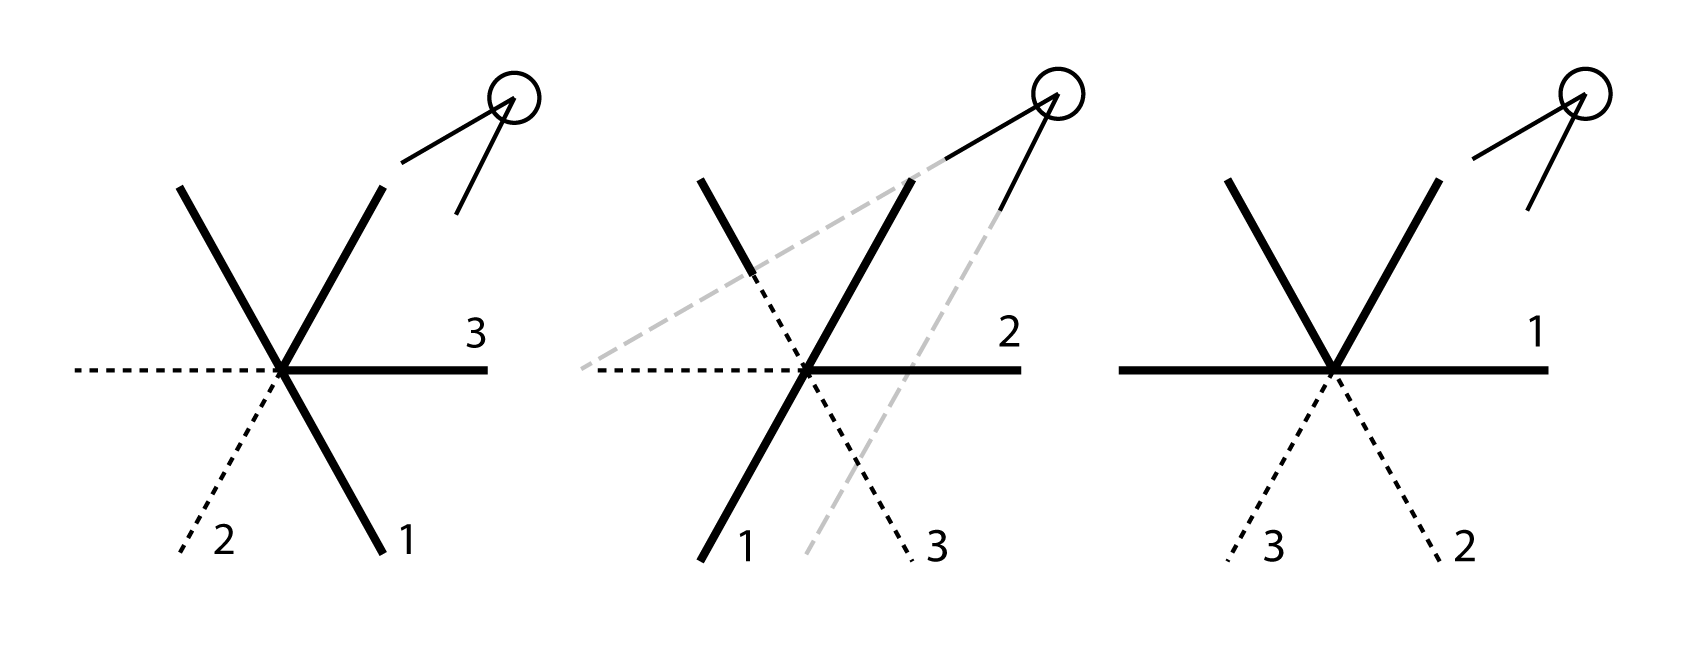
\includegraphics[width=0.6\textwidth]{./figures/LODtransparency.png}
\end{center}
\caption[Průhlednost trsu řezů]%
{Schematicky znázorněné problémy vykreslování průhledných, křížících se řezů. Tlustou plnou čarou jsou naznačeny správně vykreslené oblasti, tence čárkovaně oblasti, které nejsou vykresleny a mohou způsobit problémy.
\label{fig:lodSliceOrdering}
}
\end{figure}

Průhlednost mezi instancemi je ošetřena řazením v rámci zpracování instancí. Geometrická primitiva v rámci jedné instance je ovšem také třeba řadit. Jak je patrné z obrázku \ref{fig:lodSliceOrdering}, nelze pouhým řazením geometrických primitiv zajistit zcela korektní vykreslení. Ovšem důležité je si uvědomit skutečnost, že problémy způsobují zejména řezy skoro rovnoběžné s pohledem (dále jen \emph{rovnoběžný řez}), které jsou stejně skrývány (proto jsou vysoce průhledné). Zejména problematická je pak jejich část blíž k pozorovateli. Část dále od pozorovatele zakrývají řezy méně průhledné natočené víceméně kolmo ke směru pohledu. Stačí tedy zajistit, aby se takový rovnoběžný řez vykresloval až po ostatních.
\begin{figure}[!hbt]
\begin{center}
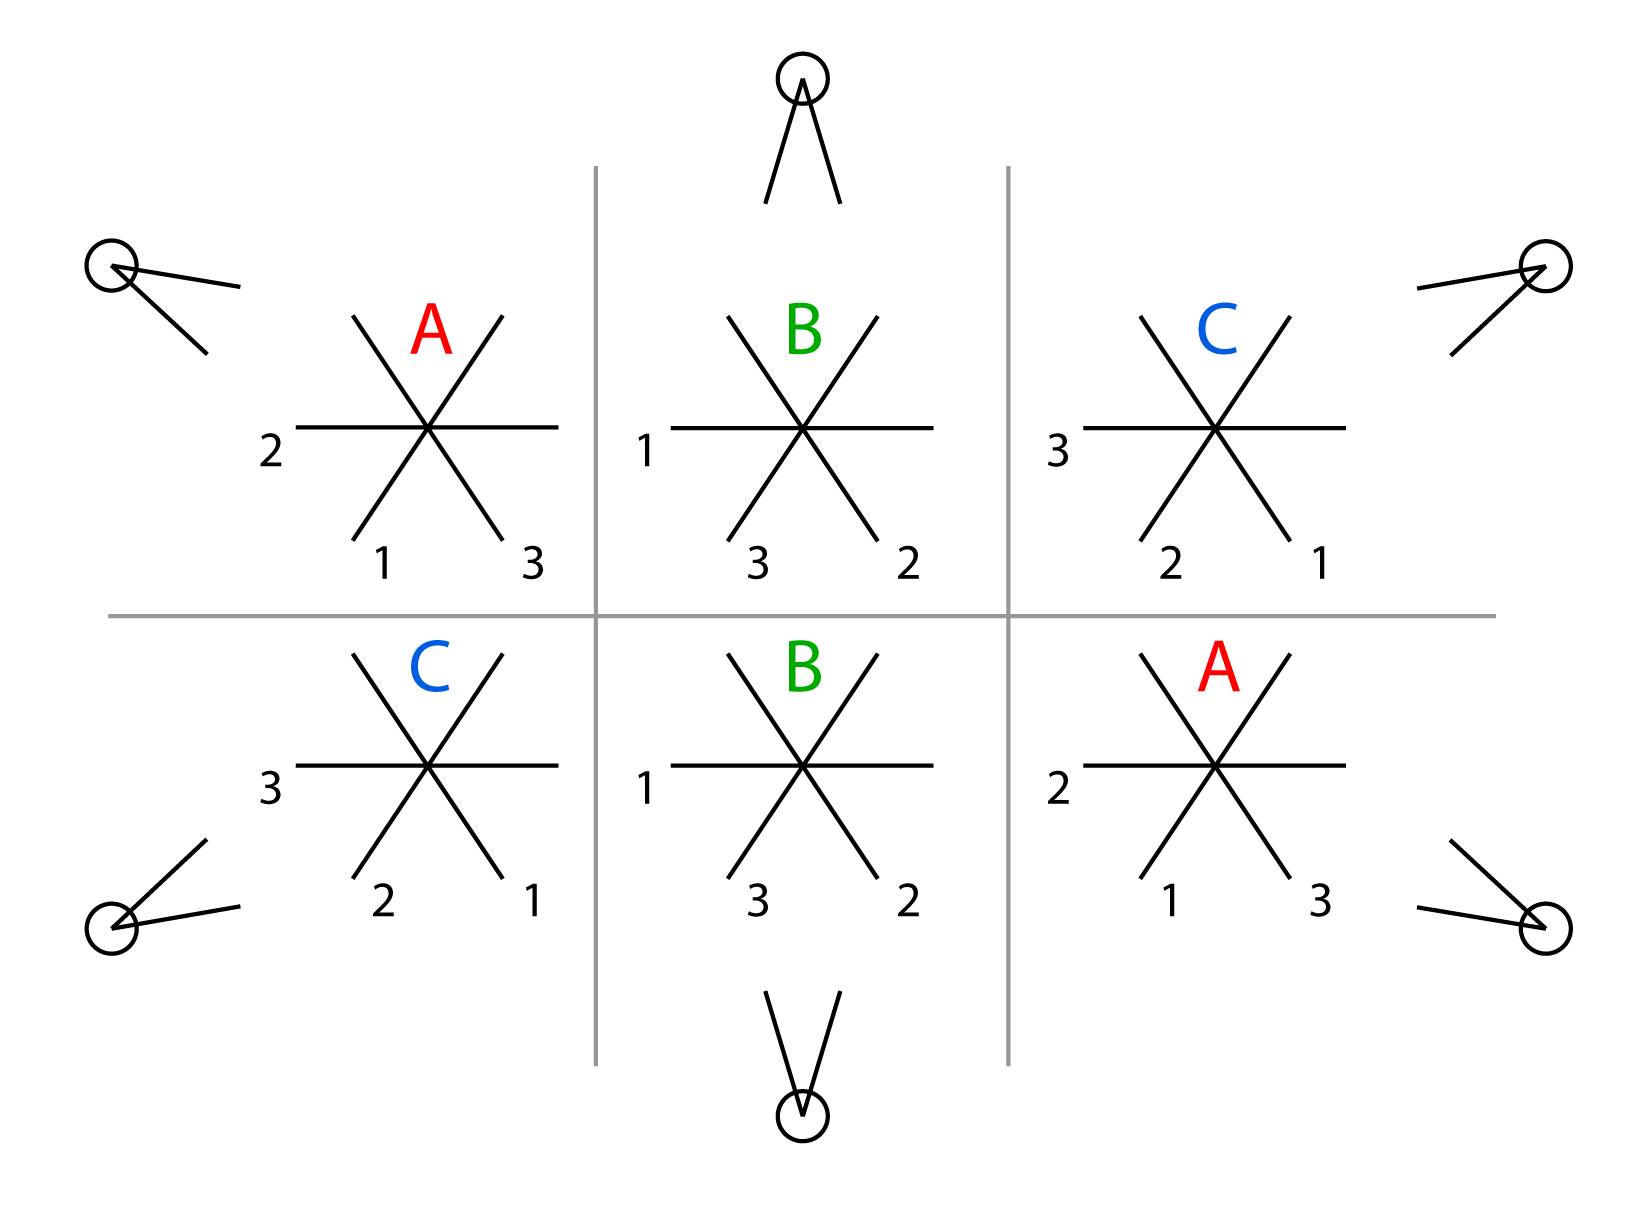
\includegraphics[width=0.6\textwidth]{./figures/LODtypes.png}
\end{center}
\caption[Variace pořadí vykreslování trsu řezů]%
{Různé případy pozice pozorovatele vůči trsu řezů. Všechny možnosti se redukují na 3 případy pořadí vykreslování řezů (A,B,C).
\label{fig:LODtypes}
}
\end{figure}
Jak je patrné z obr.~\ref{fig:LODtypes}, je třeba rozlišit, jaký případ nastává a podle toho určit pořadí vykreslení jednotlivých řezů. Fronty instancí se tedy rozpadají ještě podle tohoto kritéria (viz obr. \ref{fig:LODqueues}), neboť různé pořadí vykreslení jednotlivých řezů je zajištěno různým souborem indexů v EBO.
\begin{figure}[!hbt]
\begin{center}
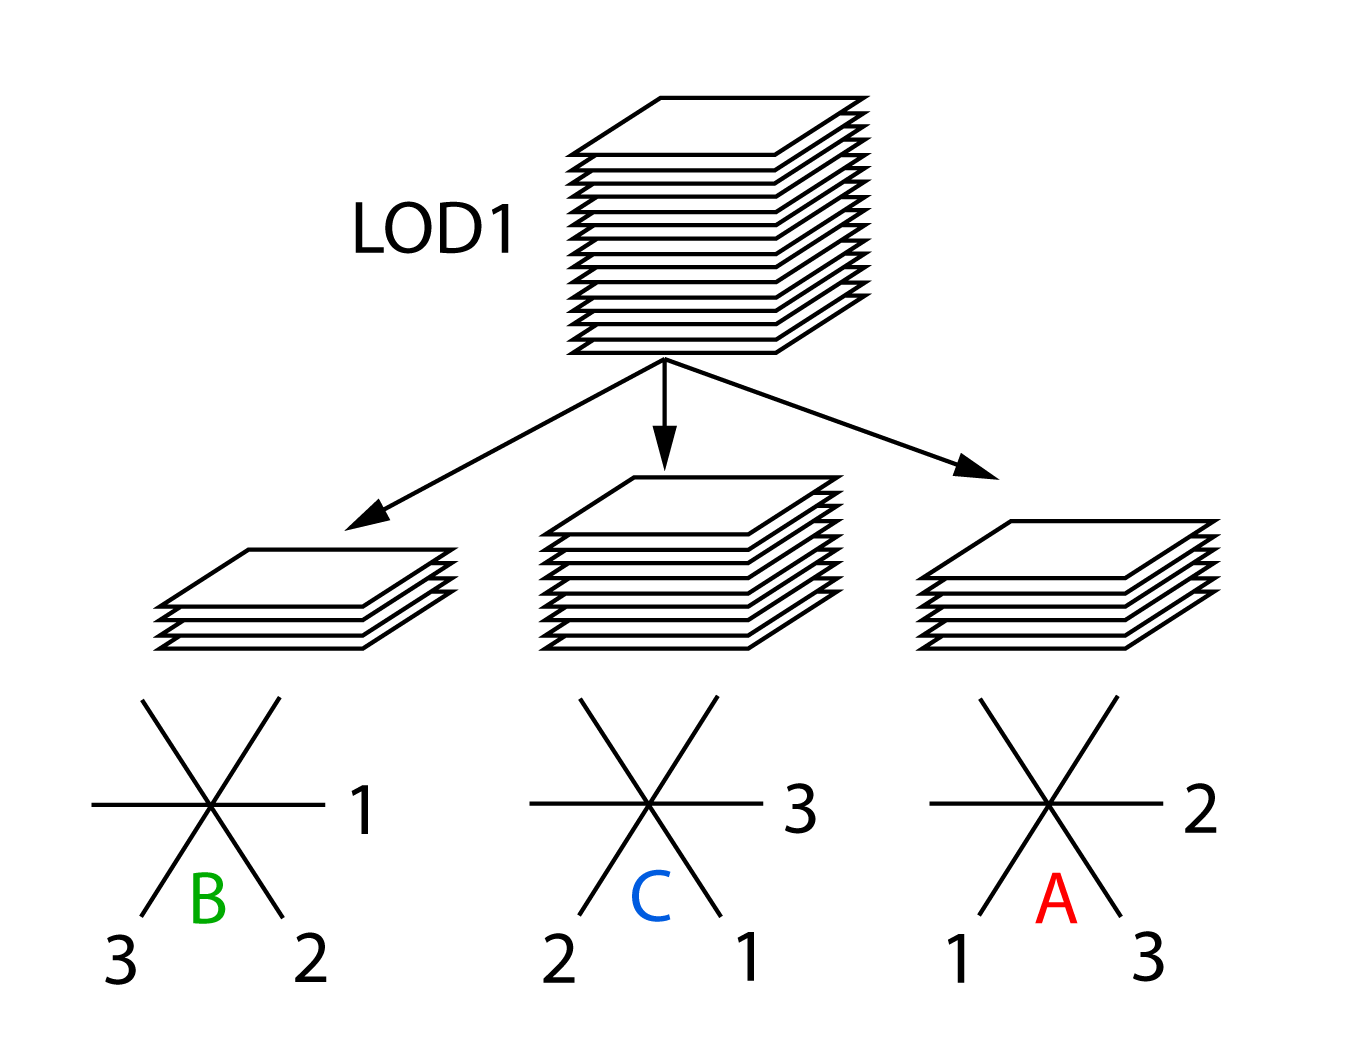
\includegraphics[width=0.4\textwidth]{./figures/renderQueuesB.png}
\end{center}
\caption[Pořadí vykreslování LOD1]%
{Rozpad fronty instancí LOD1 do několika menších front podle pořadí vykreslení (A,B,C).
\label{fig:LODqueues}
}
\end{figure}



\begin{itemize}
\item skrývání - řízení průhlednosti
\item pořadí vykreslování primitiv \& instancování (viz architektura LOD)
\item stíny
\end{itemize}
